\documentclass[12pt]{article}

\usepackage{tikz}
\usetikzlibrary{calc}

\title{An Implementation of Halfedge Data Structure in Catmull-Clark 
Subdivision for 2-Manifold Single-sided Surface}
\author{Yu Wang}
\date{August 2015}

\makeatletter
\def\BState{\State\hskip-\ALG@thistlm}
\makeatother

\begin{document}
\maketitle
\newpage

%\begin{abstract} A place for abstract later
% Contents of abstract
%\end{abstract}

\section{Introduction}
Catmull-Clark subdivision is widely applied to construct a smooth surface from an initial mesh of polygons. It is independent of the topology of initial mesh.
\section{Halfedge Data Structure} \label{sec:halfedge}

An object in the 3D Euclid space can be modeled as several meshes of polygons. For a single mesh, it comprises three types of geometry elements: vertex, edge, and face. Adjacency data structure is need to store the topological information (adjacency and connectivity) between these elements.\\
Several adjacency structures have been fully developed, including simple data structure, winged edge data structure (Baumgart, 1975), halfedge data structure (Eastman, 1982), QuadEdge Data structure (Guibas and Stolfi), and FaceEdge Data Structure (Dobkin and Laszlo, 1987).\\
Among all these data structures, the author chooses halfedge data structure in this project to realize Catmull-Clark subdivision, because 1) the storage size is independent of the mesh topology, and 2) it has a simple implementation. The author also extends its definition to add the ability in dealing with single-sided surfaces (or non-orientable object).

\subsection{Vertex, Halfedge, and Face}

The definitions and assumptions of vertex, halfedge and face follow the assumption of 2-manifold, as shown in Table \ref{table:vhfdef}. The element ID is unique. When two elements fall into the same group of element, they can not have the same ID.\\
A quadrilateral face made with four halfedges and four vertices is shown in Figure \ref{figure:singleFace}.

%Table1
\begin{table}[h]
\centering
\begin{tabular}{| l | p{0.4\textwidth} | p{0.4\textwidth}|}

\hline
		&	Definition	& Assumption	\\
\hline
Vertex	&	A 3-dimensional point.		&	No overlapping vertices 
exits in a mesh. But overlapping vertices can exist in different meshes.\\
\hline
Halfedge	&	An edge that starts from one vertex and ends at another vertex. & 
A halfedge connects exactly two non-overlapping vertices and it has a direction. 
Less than two halfedges start from the same vertex and end at the same vertex in a 
single mesh.\\
\hline
Face		&	A polygon that contains a loop of vertices and halfedges.	& A face has at 
least three non-overlapping vertices so it makes a polygon. The face has to be constructed 
with a complete loop of halfedges with on openings.\\
\hline
\end{tabular}
\caption{Definitions and assumptions of vertex, halfedge, and face} 
\label{table:vhfdef}
\end{table}

%Figure1
\begin{figure}[h]
  \centering
  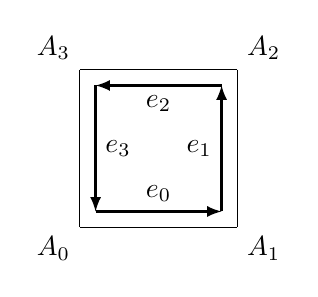
\begin{tikzpicture}
    \coordinate (A0) at (0,0);
    \coordinate (A1) at (2,0);
    \coordinate (A2) at (2,2);
    \coordinate (A3) at (0,2);
    \coordinate (B0) at (0.2,0.2);
    \coordinate (B1) at (1.8,0.2);
    \coordinate (B2) at (1.8,1.8);
    \coordinate (B3) at (0.2,1.8);
      \draw(A0)
        -- (A1) node [below right] {$A_1$};
      \draw (A1)
        -- (A2) node [above right] {$A_2$};
      \draw (A2)
        -- (A3) node [above left] {$A_3$};
      \draw (A3)
        -- (A0) node [below left] {$A_0$};
      \draw  [thick,-latex] (B0)
        -- (B1);
      \draw [thick,-latex,] (B1)
        -- (B2);
      \draw [thick,-latex,] (B2)
        -- (B3);
      \draw [thick,-latex,] (B3)
        -- (B0);
      \node [right] at (0.2, 1) {$e_3$};
      \node [above] at (1, 0.2) {$e_0$};
      \node [left] at (1.8, 1) {$e_1$};
      \node [below] at (1, 1.8) {$e_2$};
  \end{tikzpicture}
  \caption{A quadrilateral face made with four halfedges}
  \label{figure:singleFace}
\end{figure}

Elements store two categories of information: self-information and adjacency information, where the adjacency information include links in a face and links between faces. As shown in Table \ref{table:vhfInfo}. 

%Table2
\begin{table}[ht]
\centering
\begin{tabular}{| l | p{0.4\textwidth} | p{0.4\textwidth}|}

\hline
Element & Self-Information & Adjacency Information  \\
\hline
Vertex  & 1. vertex ID & 1. one outgoing halfedge   \\
& 2. vertex position & 2. on mobius connection? \\
& 3. vertex normal & \\
\hline
Halfedge & 1. edge ID & 1. start and end vertex\\
& & 2. link to parent face\\
& & 3. predecessor and successor in the parent face\\
& & 4. sibling links to adjacent face\\
& & 5. boundary links to adjacent face \\
\hline
Face    &  1. face ID & 1. one side halfedge\\
& 2. face normal &\\
\hline
\end{tabular}
\caption{Definitions and assumptions of vertex, halfedge, and face} 
\label{table:vhfInfo}
\end{table}

\subsection{Face Connections}

There are two types of face connections, the normal connection and the mobius connection, as shown in Figure \ref{figure:faceConnections}. In a typical halfedge data structure, with the assumption of double-sided surface, the pair of halfedges between two faces are defined with opposite direction. The author extends this idea to single-sided surface and adds another type of connection, named as mobius connection. In a mobius connection, the pair of halfedges are in same direction. In the example of Figure \ref{figure:faceConnections}, on the top, $e_1$ and $e_1'$ are siblings to each other. On the bottom, $e_1$ and $e_1'$ are mobius siblings to each other.

%Figure2
\begin{figure}[ht]
  \centering
  %Normal Junction
  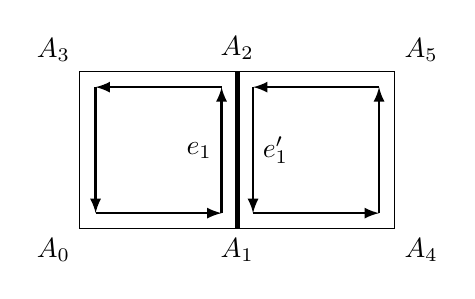
\begin{tikzpicture}
    \coordinate (A0) at (0,0);
    \coordinate (A1) at (2,0);
    \coordinate (A2) at (2,2);
    \coordinate (A3) at (0,2);
    \coordinate (A4) at (4,0);
    \coordinate (A5) at (4,2);
    \coordinate (B0) at (0.2,0.2);
    \coordinate (B1) at (1.8,0.2);
    \coordinate (B2) at (1.8,1.8);
    \coordinate (B3) at (0.2,1.8);
    \coordinate (B4) at (2.2,0.2);
    \coordinate (B5) at (3.8,0.2);
    \coordinate (B6) at (3.8,1.8);
    \coordinate (B7) at (2.2,1.8);
      \draw(A0) -- (A1) node [below] {$A_1$};
      \draw [ultra thick] (A1) -- (A2) node [above] {$A_2$};
      \draw (A2) -- (A3) node [above left] {$A_3$};
      \draw (A3) -- (A0) node [below left] {$A_0$};
      \draw (A1) -- (A4) node [below right] {$A_4$};
      \draw (A4) -- (A5) node [above right] {$A_5$};
      \draw (A5) -- (A2);
      \draw  [thick,-latex] (B0)
        -- (B1);
      \draw [thick,-latex,] (B1)
        -- (B2);
      \draw [thick,-latex,] (B2)
        -- (B3);
      \draw [thick,-latex,] (B3)
        -- (B0);
      \draw  [thick,-latex] (B4)
        -- (B5);
      \draw [thick,-latex,] (B5)
        -- (B6);
      \draw [thick,-latex,] (B6)
        -- (B7);
      \draw [thick,-latex,] (B7)
        -- (B4);
      \node [left] at (1.8, 1) {$e_1$};
      \node [right] at (2.2, 1) {$e_1'$};
  \end{tikzpicture}
  
  %Mobius Junction
  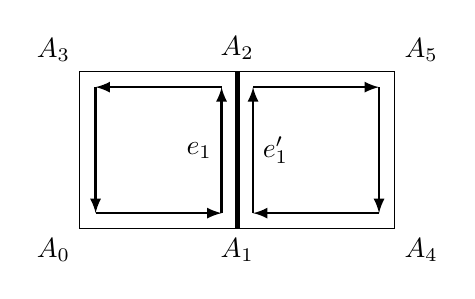
\begin{tikzpicture}
    \coordinate (A0) at (0,0);
    \coordinate (A1) at (2,0);
    \coordinate (A2) at (2,2);
    \coordinate (A3) at (0,2);
    \coordinate (A4) at (4,0);
    \coordinate (A5) at (4,2);
    \coordinate (B0) at (0.2,0.2);
    \coordinate (B1) at (1.8,0.2);
    \coordinate (B2) at (1.8,1.8);
    \coordinate (B3) at (0.2,1.8);
    \coordinate (B4) at (2.2,0.2);
    \coordinate (B5) at (3.8,0.2);
    \coordinate (B6) at (3.8,1.8);
    \coordinate (B7) at (2.2,1.8);
      \draw(A0) -- (A1) node [below] {$A_1$};
      \draw [ultra thick] (A1) -- (A2) node [above] {$A_2$};
      \draw (A2) -- (A3) node [above left] {$A_3$};
      \draw (A3) -- (A0) node [below left] {$A_0$};
      \draw (A1) -- (A4) node [below right] {$A_4$};
      \draw (A4) -- (A5) node [above right] {$A_5$};
      \draw (A5) -- (A2);
      \draw  [thick,-latex] (B0)
        -- (B1);
      \draw [thick,-latex,] (B1)
        -- (B2);
      \draw [thick,-latex,] (B2)
        -- (B3);
      \draw [thick,-latex,] (B3)
        -- (B0);
      \draw  [thick,-latex] (B5)
        -- (B4);
      \draw [thick,-latex,] (B4)
        -- (B7);
      \draw [thick,-latex,] (B7)
        -- (B6);
      \draw [thick,-latex,] (B6)
        -- (B5);
      \node [left] at (1.8, 1) {$e_1$};
      \node [right] at (2.2, 1) {$e_1'$};
  \end{tikzpicture}
  \caption{Normal connection (up) and mobius connection (bottom) between two faces}
  \label{figure:faceConnections}
\end{figure}

\subsection{Traversals} 
Two basic traversals are necessary to implement Catmull-Clark subdivision: 1) traversal around a face, and 2) traversal around a vertex.
\subsubsection{Traversal Around Face}
The traversal around a face lead to all the edges and vertices belong to this face. It starts from one side halfedge, follows the halfedge flow, and ends at the halfedge that the face traverse starts.
Traversal of all faces in a mesh takes O(F) time, where F is the total number of faces in the mesh.
\subsubsection{Traversal Around Vertex}
The traversal around a vertex lead to all the edges and faces that contains this vertex. The traversal of a vertex need to consider two issues: 1) is this vertex on a boundary, and  2) is this vertex on a mobius connection. This makes four different types of vertex traversals. See Figure \ref{figure:traversalAroundVertexNormal} - \ref{figure:traversalAroundVertexMobiusB} for examples.

In the vertex traversal without boundary and mobius issue, we start from one outgoing halfedge of this vertex. We continue to go to the next outgoing halfedge by going to the successor of its sibling until we hit the first outgoing halfedge. In the example of Figure \ref{figure:traversalAroundVertexNormal}, if start and end at halfedge $e_1$, the sequence of traversal is: $e_1$ (sibling link to) $e_1'$ (successor link to) $e_2$ (sibling link to) $e_2'$ (successor link to) $e_3$ (sibling link to) $e_3'$ (successor link to) $e_4$ (sibling link to ) $e_4'$  (successor link to)  $e_1$.

In order to address the issue of a vertex on boundary, instead of using sibling links, we use boundary links. In the example of Figure \ref{figure:traversalAroundVertexNormalB}, we have a boundary $e_4'$ to $e_2$. If start and end at halfedge $e_1$, the sequence of traversal is: $e_1$ (sibling link to) $e_1'$ (successor link to) $e_2$ (boundary link to) $e_4'$ (successor link to)  $e_1$.

To address the issue of vertex on a mobius connection, instead of using normal links, we use mobius links. At the same time, we switch between the successor and predecessor to the sibling every time we hit a mobius connection.  In the example of Figure \ref{figure:traversalAroundVertexNormal}, $e_1$ to $e_1'$ and $e_3$ to $e_3'$ have mobius siblings rather than normal sibling. If start and end at halfedge $e_1$, the sequence of traversal is: $e_1$ (mobius sibling link to) $e_1'$ (predecessor link to) $e_2$ (sibling link to) $e_2'$ (predecessor link to) $e_3$ (mobius sibling link to) $e_3'$ (successor link to) $e_4$ (sibling link to ) $e_4'$  (successor link to)  $e_1$.

If boundary and mobius connection both occur, we use a combination of the two methods above. In the example of Figure \ref{figure:traversalAroundVertexNormal}, $e_1$ to $e_1'$ and $e_3$ to $e_3'$ have mobius siblings rather than normal sibling and we have a mobius boundary connection between $e_4'$ and $e_2$. If start end end at halfedge $e_1$, the sequence of traversal is: $e_1$ (mobius sibling link to) $e_1'$ (predecessor link to) $e_2$ (mobius boundary link to ) $e_4'$  (successor link to)  $e_1$.

We can combine the four cases together as shown in Algorithm 1.

%Figure3
\begin{figure}[ht]
  \centering
  %Normal Junction
  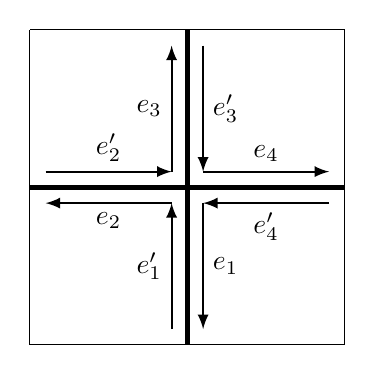
\begin{tikzpicture}
    \coordinate (A0) at (0,0);
    \coordinate (A1) at (2,0);
    \coordinate (A2) at (2,2);
    \coordinate (A3) at (0,2);
    \coordinate (A4) at (4,0);
    \coordinate (A5) at (4,2);
    \coordinate (A6) at (4,4);
    \coordinate (A7) at (2,4);
    \coordinate (A8) at (0,4);
    
    \coordinate (B0) at (0.2,0.2);
    \coordinate (B1) at (1.8,0.2);
    \coordinate (B2) at (1.8,1.8);
    \coordinate (B3) at (0.2,1.8);
    \coordinate (B4) at (2.2,0.2);
    \coordinate (B5) at (3.8,0.2);
    \coordinate (B6) at (3.8,1.8);
    \coordinate (B7) at (2.2,1.8);
    \coordinate (B8) at (0.2,2.2);
    \coordinate (B9) at (1.8,2.2);
    \coordinate (B10) at (1.8,3.8);
    \coordinate (B11) at (0.2,3.8);
    \coordinate (B12) at (2.2,2.2);
    \coordinate (B13) at (3.8,2.2);
    \coordinate (B14) at (3.8,3.8);
    \coordinate (B15) at (2.2,3.8);

     \draw (A0) -- (A1);
     \draw [ultra thick](A1) -- (A2);
     \draw  [ultra thick](A2) -- (A3);
     \draw (A3) -- (A0);
     \draw (A1) -- (A4);
     \draw (A4) -- (A5);
     \draw [ultra thick](A5) -- (A2);
     \draw (A3) -- (A8);
     \draw (A8) -- (A7);
     \draw (A7) -- (A6);
     \draw (A6) -- (A5);
     \draw [ultra thick] (A7) -- (A2);

     \draw [thick,-latex,] (B1) -- (B2);
     \draw [thick,-latex,] (B2) -- (B3);
     \draw [thick,-latex,] (B6) -- (B7);
     \draw [thick,-latex,] (B7) -- (B4);
     \draw [thick,-latex,] (B8) -- (B9);
     \draw  [thick,-latex] (B9) -- (B10);
     \draw [thick,-latex,] (B15) -- (B12);
     \draw [thick,-latex,] (B12) -- (B13);
     \node [left] at (1.8, 1) {$e_1'$};
     \node [right] at (2.2, 1) {$e_1$};
     \node [left] at (1.8, 3) {$e_3$};
     \node [right] at (2.2, 3) {$e_3'$};
     \node [below] at (1, 1.8) {$e_2$};
     \node [above] at (1, 2.2) {$e_2'$};
     \node [below] at (3, 1.8) {$e_4'$};
     \node [above] at (3, 2.2) {$e_4$};
  \end{tikzpicture}
  \caption{Vertex traversal without boundary and without moibus connection}
  \label{figure:traversalAroundVertexNormal}
\end{figure}
%Figure 4
\begin{figure}[ht]
  \centering
  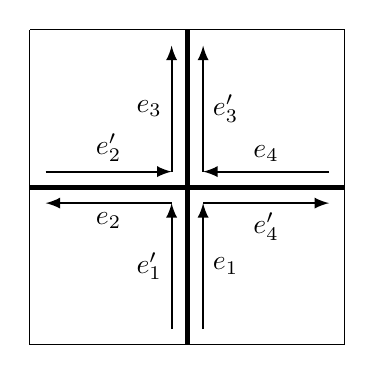
\begin{tikzpicture}
    \coordinate (A0) at (0,0);
    \coordinate (A1) at (2,0);
    \coordinate (A2) at (2,2);
    \coordinate (A3) at (0,2);
    \coordinate (A4) at (4,0);
    \coordinate (A5) at (4,2);
    \coordinate (A6) at (4,4);
    \coordinate (A7) at (2,4);
    \coordinate (A8) at (0,4);
    
    \coordinate (B0) at (0.2,0.2);
    \coordinate (B1) at (1.8,0.2);
    \coordinate (B2) at (1.8,1.8);
    \coordinate (B3) at (0.2,1.8);
    \coordinate (B4) at (2.2,0.2);
    \coordinate (B5) at (3.8,0.2);
    \coordinate (B6) at (3.8,1.8);
    \coordinate (B7) at (2.2,1.8);
    \coordinate (B8) at (0.2,2.2);
    \coordinate (B9) at (1.8,2.2);
    \coordinate (B10) at (1.8,3.8);
    \coordinate (B11) at (0.2,3.8);
    \coordinate (B12) at (2.2,2.2);
    \coordinate (B13) at (3.8,2.2);
    \coordinate (B14) at (3.8,3.8);
    \coordinate (B15) at (2.2,3.8);

     \draw (A0) -- (A1);
     \draw [ultra thick](A1) -- (A2);
     \draw  [ultra thick](A2) -- (A3);
     \draw (A3) -- (A0);
     \draw (A1) -- (A4);
     \draw (A4) -- (A5);
     \draw [ultra thick](A5) -- (A2);
     \draw (A3) -- (A8);
     \draw (A8) -- (A7);
     \draw (A7) -- (A6);
     \draw (A6) -- (A5);
     \draw [ultra thick] (A7) -- (A2);

     \draw [thick,-latex,] (B1) -- (B2);
     \draw [thick,-latex,] (B2) -- (B3);
     \draw [thick,-latex,] (B7) -- (B6);
     \draw [thick,-latex,] (B4) -- (B7);
     \draw [thick,-latex,] (B8) -- (B9);
     \draw [thick,-latex] (B9) -- (B10);
     \draw [thick,-latex,] (B13) -- (B12);
     \draw [thick,-latex,] (B12) -- (B15);
     \node [left] at (1.8, 1) {$e_1'$};
     \node [right] at (2.2, 1) {$e_1$};
     \node [left] at (1.8, 3) {$e_3$};
     \node [right] at (2.2, 3) {$e_3'$};
     \node [below] at (1, 1.8) {$e_2$};
     \node [above] at (1, 2.2) {$e_2'$};
     \node [below] at (3, 1.8) {$e_4'$};
     \node [above] at (3, 2.2) {$e_4$};  \end{tikzpicture}
  \caption{Vertex traversal without boundary and with moibus connection}
  \label{figure:traversalAroundVertexMobius}
\end{figure}
%Figure4
\begin{figure}[ht]
  \centering
  %Normal Junction
  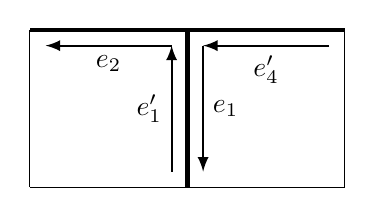
\begin{tikzpicture}
    \coordinate (A0) at (0,0);
    \coordinate (A1) at (2,0);
    \coordinate (A2) at (2,2);
    \coordinate (A3) at (0,2);
    \coordinate (A4) at (4,0);
    \coordinate (A5) at (4,2);
    
    \coordinate (B0) at (0.2,0.2);
    \coordinate (B1) at (1.8,0.2);
    \coordinate (B2) at (1.8,1.8);
    \coordinate (B3) at (0.2,1.8);
    \coordinate (B4) at (2.2,0.2);
    \coordinate (B5) at (3.8,0.2);
    \coordinate (B6) at (3.8,1.8);
    \coordinate (B7) at (2.2,1.8);

     \draw (A0) -- (A1);
     \draw [ultra thick](A1) -- (A2);
     \draw  [ultra thick](A2) -- (A3);
     \draw (A3) -- (A0);
     \draw (A1) -- (A4);
     \draw (A4) -- (A5);
     \draw [ultra thick](A5) -- (A2);

     \draw [thick,-latex,] (B1) -- (B2);
     \draw [thick,-latex,] (B2) -- (B3);
     \draw [thick,-latex,] (B6) -- (B7);
     \draw [thick,-latex,] (B7) -- (B4);
     
     \node [left] at (1.8, 1) {$e_1'$};
     \node [right] at (2.2, 1) {$e_1$};
     \node [below] at (1, 1.8) {$e_2$};
     \node [below] at (3, 1.8) {$e_4'$};
  \end{tikzpicture}
  \caption{Vertex traversal withboundary and without moibus connection}
  \label{figure:traversalAroundVertexNormalB}
\end{figure}

%Figure5
\begin{figure}[ht]
  \centering
  %Normal Junction
  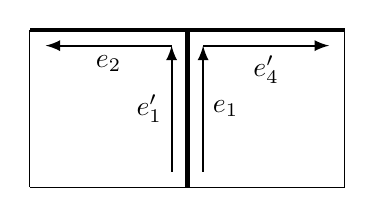
\begin{tikzpicture}
    \coordinate (A0) at (0,0);
    \coordinate (A1) at (2,0);
    \coordinate (A2) at (2,2);
    \coordinate (A3) at (0,2);
    \coordinate (A4) at (4,0);
    \coordinate (A5) at (4,2);
    
    \coordinate (B0) at (0.2,0.2);
    \coordinate (B1) at (1.8,0.2);
    \coordinate (B2) at (1.8,1.8);
    \coordinate (B3) at (0.2,1.8);
    \coordinate (B4) at (2.2,0.2);
    \coordinate (B5) at (3.8,0.2);
    \coordinate (B6) at (3.8,1.8);
    \coordinate (B7) at (2.2,1.8);

     \draw (A0) -- (A1);
     \draw [ultra thick](A1) -- (A2);
     \draw  [ultra thick](A2) -- (A3);
     \draw (A3) -- (A0);
     \draw (A1) -- (A4);
     \draw (A4) -- (A5);
     \draw [ultra thick](A5) -- (A2);

     \draw [thick,-latex,] (B1) -- (B2);
     \draw [thick,-latex,] (B2) -- (B3);
     \draw [thick,-latex,] (B7) -- (B6);
     \draw [thick,-latex,] (B4) -- (B7);
     
     \node [left] at (1.8, 1) {$e_1'$};
     \node [right] at (2.2, 1) {$e_1$};
     \node [below] at (1, 1.8) {$e_2$};
     \node [below] at (3, 1.8) {$e_4'$};

  \end{tikzpicture}
  \caption{Vertex traversal with boundary and with moibus connection}
  \label{figure:traversalAroundVertexMobiusB}
\end{figure}

\subsection{Mesh Construction}
The input of Catmull-Clark is a polygon mesh with arbitrary topology.
\subsubsection{Build from Elements}
\subsubsection{Instantiation and Rotation}
\subsubsection{Build by Merging Meshes}

\section{Catumll-Clark Subdivision} \label{sec:ccsd}

\subsection{General Approach of Catmull-Clark Subdivision}

\subsubsection{Compute Vertex Positions of New Mesh}

\subsubsection{Make Connections of New Mesh}

\subsection{Sharp Crease and Boundary Feature}

\subsection{Mobius Connection}

\section{Offset Surface} \label{sec:offset}

\subsection{Compute Vertex Normals}

\subsection{Positive and Negative Offsets}

\subsection{Mobius Connection Issue}

\section{Input and Output}

\section{Test Cases and Discussions}

\section{Future Researches}


\end{document}